\documentclass[authoryearcitations]{UoYCSproject}
\usepackage{todonotes}

\SetExtraKerning
   [unit = space]%
   {encoding = *}%
   {\ = {500,}}

\author{Joshua Goodwin}
\title{Layout of arguments in the Artoo tool}
% \date{}
\supervisor{}
\BEng

\wordcount{?}

% \includes{Appendices \ref{cha:usefulpackages}, \ref{cha:gotchas} and
  % \ref{cha:deptfac}}

% \excludes{\autoref{cha:quoteex}}

\abstract{}

% \dedication{To}

% \acknowledgements{
%   I would like to thank
% }

\begin{document}

\maketitle

% \listoffigures
% \listoftables
% \renewcommand*{\lstlistlistingname}{List of Listings}
% \lstlistoflistings

% \cleardoublepage

% \part{Preliminaries}
% \label{sec:start}
% \thispagestyle{empty}\cleardoublepage

%%%%%%%%%%%%%%%%%%%%%%%%%%%%%%%%%%%%%%%%%%%%%%%%%%%%%%%%%%%

\chapter{Introduction?}


\section{The Goal Structuring Notation}

The Goal Structuring Notation (GSN) is a graphical agumentation notation.
It allows logical arguments - in particular, safety arguments, which \ldots  - to be represented explicitly, in a much clearer way than textual arguments allow.

GSN arguments are directed, multivariate \todo{I think}, hierachical graphs.

An argument begins with a single, main goal or claim\todo{two words used interchangably\ldots}. rectangle

Nodes within GSN arguments contain text, and represent ``claims, strategies, evidence, and context/assumption/justification annotations'';
edges represent relationships between these.

\begin{description}
    \item[Goal/claim]
    a statement that can be assessed to be true or false
    \item[Strategy]
\end{description}

\begin{figure}
    \centering
    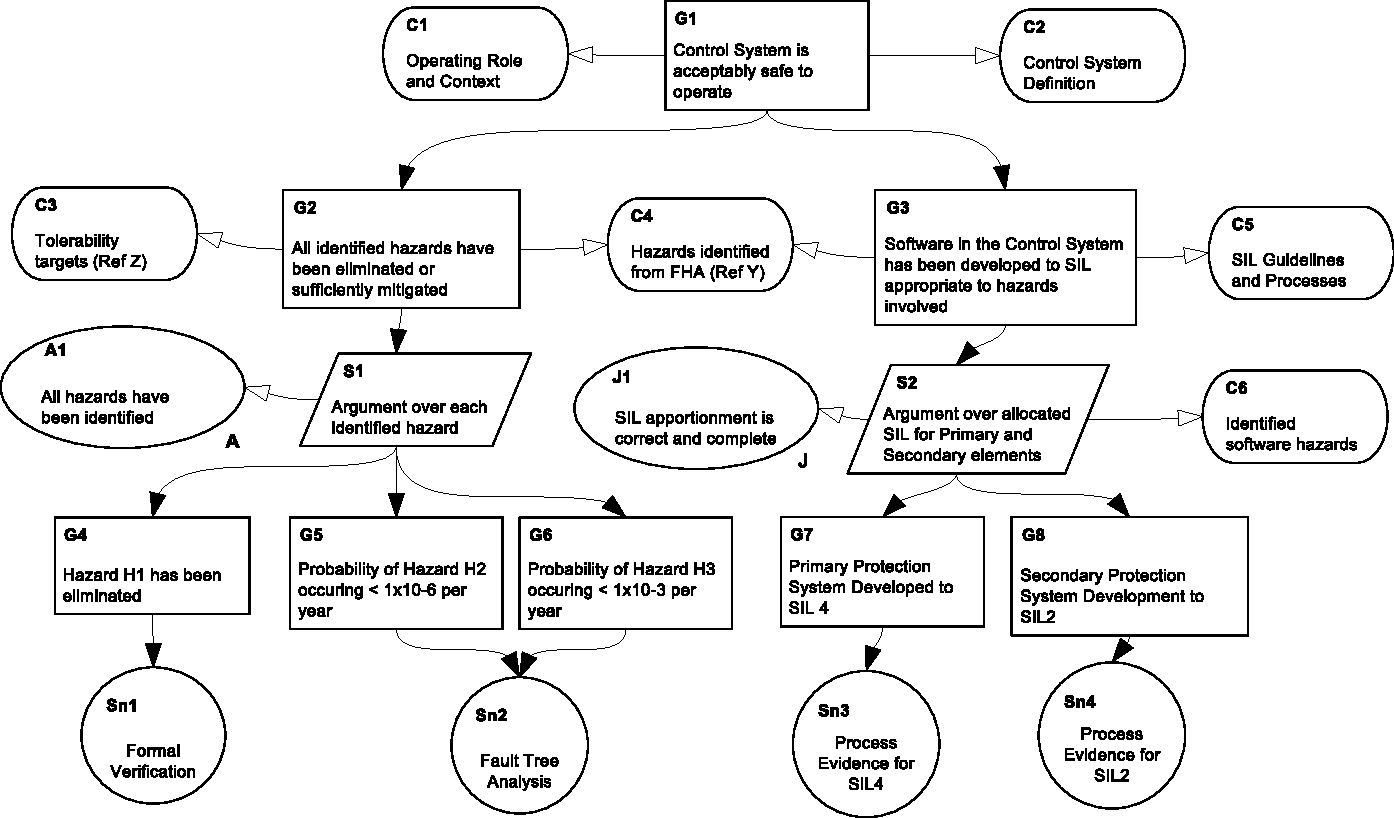
\includegraphics[width=\textwidth]{example_argument.pdf}
    \caption{An example argument, from the GSN specification [I don't think this layout is very good, because\ldots]    }
\end{figure}

\ldots

other notations: Connt

\section{Artoo}

Artoo (Argumentation Tool) is a web-based tool intended for drawing GSN arguments.

\ldots

other tools also exist for drawing GSN argments.

\begin{figure}
    \centering
    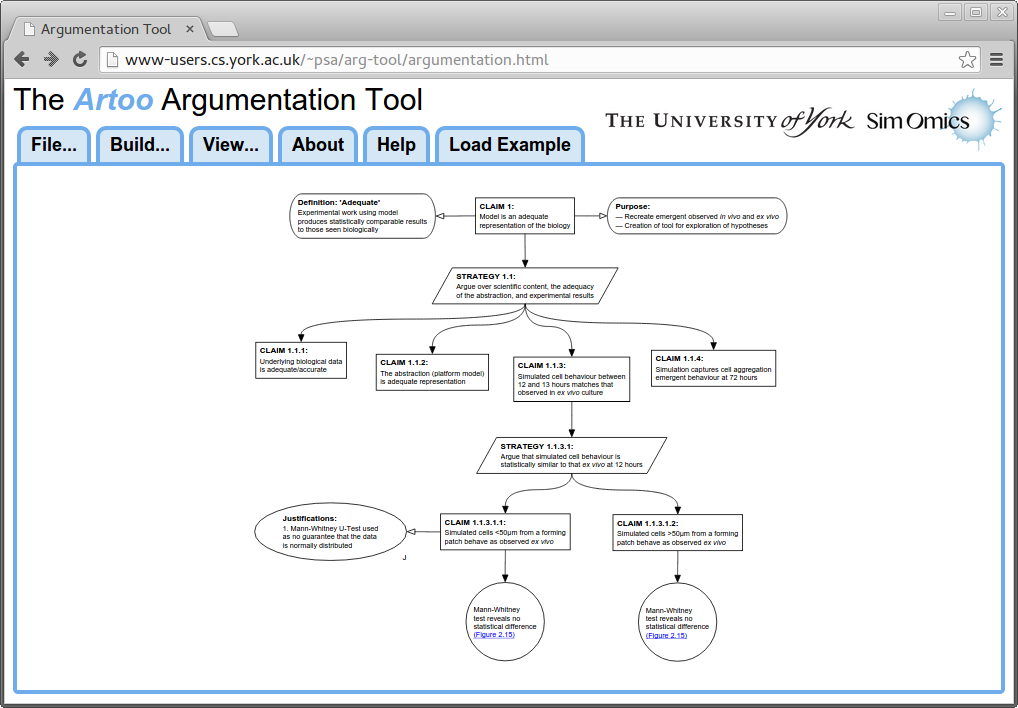
\includegraphics[width=\textwidth]{graphics/artoo_screenshot.png}
    \caption{The Artoo tool, displaying an argument }
\end{figure}

\todo{use the same argument as in the naked dexample?}

\section{[what I'm going to do]}

This [report/project/thing] will \ldots

    \begin{enumerate}
        \item \begin{itemize}
            \item ,
        \end{itemize}
    \end{enumerate}

\subsection{Problem definition?}

Input:

as I said earlier

\subsection{Problem definition?}

Artoo also allows the drawing of invalid GSN argments ...
if the graph layout [thing] is to be executed every time the graph is edited, then it must accept these .
If the algorithm [is exposed to the user by a] button, then there is the poissibility of checking 

\subsubsection{\ldots}

Already, Artoo only works a limited set of web browsers: recent versions of \ldots
The features added in this project will not interact with the browser in any new way -- only needing to change the position of nodes, using functions already in the code -- it is very unlikely that there will be any problems \ldots



\chapter{Literature review}

\section{A brief history}

In 1736, \citet{euler} solved the Seven Bridges of Ka\"{o}nigsberg problem by drawing a graph.
\citet{ismail2009some}
\todo{a strange paper to choose. perhaps multiple citations?}
pinpoint his use of this method as the birth of graph theory.

In 1963, \citet{tutte} popularised the problem of graph drawing when he presented 


["who showed that polyhedral graphs may be drawn in the plane with all faces convex by fixing the vertices of the outer face of a planar embedding of the graph into convex position, placing a spring-like attractive force on each edge, and letting the system settle into an equilibrium"]

Perhaps his most relevant \ldots was the idea of modelling the graph as a system of springs and masses \ldots 

In the same year, \citet{Knuth63} described a system for drawing flowcharts that describe algorithms. \citet{battista} \todo{find out page number!} says this is [the first example of an algorithm for visualising information] although \citeauthor{Knuth63} cites earlier work done on a similar system by \citet{haibt1959}.




\ldots

\citet{huang2007effects} divide graphs into two groups: abstract graphs and domain graphs.
GSN arguments fall into the latter category \ldots  therefore \ldots
\todo{I don't think this is widely agreed upon}


\section{What makes a good graph layout?}

Speed is an obvious desirable property of any 

GSN was intended to be clearer than textual arguments \ldots

The Gestalt principles of visual perception, based on the wider Gestalt theory of the mind developed by German psychologists of the Berlin School in the late 19th and early 20th centuries, are sometimes [?] used to [inform/justify?] heuristics

The principle 

Some studies have tried \ldots cognitive effects [Purchase et al?]

\subsection{Edge crossings}

There can be many practical motivations for minimising edge crossings.
When P\`{a}l Tur\`{a}n worked in a brick factory during World War II,
he wondered about the minumum number of crossings in a graph representing
brick kilns, storage sites and the paths between them \ldots
When a graph represents an electrical circuit, the  

[But] more relevantly [which studies?] have found that edge crossings is the most important factor for comprehension

[who?] found that using the Gestalt principle of `closure' \ldots the viewer's mind instinctively joins up the lines

\section{approaches?}

\subsection{force dire}

\ldots a successor to \citet{tutte} spring embedding

[gansner 199*]

\subsection{grid}



\subsection{force dire}

\section{[GSN-/Artoo-specific considerations?]}

[move to Requirements?]

The GSN specification \citep[section~2.2, pp.~26--27]{gsnstandard} gives some guidance on the layout of arguments \ldots



\subsection{Dangling edges}

suggests incomplete graph

\subsection{Directed cycles}

It can be useful to remove directed cycles from the internal representation of a graph
(before drawing them back in their correct, original directions)
-- for example, in order to assign a consistent rank to each node.
This is achieved by reversing certain edges.
\citet{gansner1993} show that a simple depth-first-search \ldots  Minimising the number of edges is more difficult, \citeauthor{gansner1993} \ldots

\subsection{Undirected cycles}

Undirected cycles can be elimiated by ignoring certain edges altogether, to produce a tree.  [citation needed]



\section{[Alternatives to JavaScript]}

Various [things] have been developed in response to percieved shortcomings in JavaScript \ldots

Programs written in the CoffeeScript\footnote{\url{http://coffeescript.org/}} language, designed to be more succinct and with some extra features, can be transcompiled to JavaScript \ldots this is interesting but \ldots

Brython \footnote{\url{http://www.brython.info/}} is a Python 3 interpreter written in JavaScript that can run in a web browser. \todo{performance overhead etc\ldots}

Haste\footnote{\url{http://haste-lang.org/}}, UHC-JS\footnote{\url{http://uu-computerscience.github.io/uhc-js/}} and GHCJS\footnote{} are compilers from Haskell to JavaScript; SMLtoJS\footnote{\url{http://www.smlserver.org/smltojs/}} is a Standard ML--to-JavaScript compiler. These are perhaps most interesting [?], since \citet{kennedyfuntrees} observed that a tree layout algorithm implemented in Standard ML ``reflects the structure of the abstract solution much better than an imperative language implementation''.



ASM\footnote{} is a strict subset of 

[However]


\section{Software development methodologies}

In \citeyear{67poorslop}, \citet*{67poorslop} explained ``Why Programming is a Good Medium for Expressing Poorly Understood and Sloppily Formulated Ideas''.
(More recently, [sussman] gave a talk with the same title \ldots \todo{\url{http://vimeo.com/12060509}}.)


\section{}

Reuse of existing software libraries is widely [?] understood to be [a very sensible idea]. There are , which \ldots for comparison with 

\begin{description}
    \item[Springy] is
    \item[Arbor] is an implementation of the Barnes-Hut algorithm for 
    \item[The JavaScript InfoVis Toolkit] contains algorithms ported from \ldots
    \item[vis.js]
\end{description}

The Graphviz library contains several algorithms, including \ldots [as described in \ldots]. Although it is written in C, Emscripten \footnote{\url{http://emscripten.org}} can compile LLVM bitcode (readily compiled from C code) [as described earlier?] to the ASM subset of JavaScript -

These implementations also provide lessons on the structure of \ldots



\bibliography{report}

% appendices go here

\end{document}
